\section*{Введение}

В жизненном цикле программного обеспечения важную роль занимает этап
поддержки\cite{maintance}. Этот этап по разным оценкам
составляет от 30 до 80\% общего бюджета проекта. Поэтому для
промышленного программного кода важно, чтобы его было легко читать и изменять.
Рассмотрим описание функций
на рис.~\ref{fig:wikiExUnfor} и \ref{fig:wikiExBSD}.

\begin{figure}[h!]
	\centering
	\lstinputlisting[language=C]{codes/wikiExUnfor.c}
	\caption{Неформатированный код}
	\label{fig:wikiExUnfor}
\end{figure}

\begin{figure}[h!]
	\centering
	\lstinputlisting[language=C]{codes/wikiExBSD.c}
  \caption{Форматированный код (BSD)}
	\label{fig:wikiExBSD}
\end{figure}

Эти функции семантически и синтаксически эквиваленты с точки зрения
компилятора C, но вариант, приведенный на
рис.~\ref{fig:wikiExUnfor}, гораздо хуже
поддается понимаю человека и требует большего времени на изменение,
что увеличивает стоимость и трудозатраты на поддержку. Как мы видим из этого
примера, программные тексты должны явным образом отражать
структуру синтаксического дерева программы.

Кроме того, распространенной практикой~\cite{codingStandarts},
доказавшей свою состоятельность, является использования
общепроектного стандарта кодирования (\emph{coding convention}).
\emph{Стандарт кодирования (СК)} ---
это набор соглашений, которые используются
при написании программного кода. В него входят: способы выбора имен переменных
и других идентификаторов, стили отступов при оформлении логических блоков,
способы расстановки ограничителей логических блоков (скобок),
формат комментариев. СК также призван упростить анализ и изменение
программы, поэтому его важно соблюдать, что вводит
дополнительные ограничения на исходные тексты. СК разных проектов, даже
реализуемых на одном и том же языке программирования, могут существенно
различаться.
Так код на рис.~\ref{fig:wikiExBSD} соответствует СК
BSD \footnote{\cd{http://www.freebsd.org/cgi/man.cgi?query=style\&sektion=9}},
а на рис.~\ref{fig:wikiExGNU} ---
GNU\footnote{\cd{http://www.gnu.org/prep/standards/standards.pdf}}.

\begin{figure}[h!]
	\centering
	\lstinputlisting[language=C]{codes/wikiExGNU.c}
  \caption{Форматированный код (GNU)}
	\label{fig:wikiExGNU}
\end{figure}

Кроме ситуаций, когда СК в проекте поддерживается при ручном написании
программного кода, существует другой важный пример использования СК ---
в языковых процессорах. \emph{Языковой процессор} (\emph{ЯП}) ---
это программное средство, принимающее на вход программу в виде текста
на некотором языке (программирования, разметки и т. д.) и решающее
определенную задачу над этой программой. К языковым процессорам можно
отнести: компиляторы, суперкомпиляторы, интерпретаторы,
средства статического анализа кода, декомпиляторы, средства рефакторинга,
средства реинжиниринга, интегрированные среды разработки (IDE) и др.

Первым этапом работы ЯП является \emph{синтаксический анализ}, то есть
сопоставление входного текста (линейной последовательности лексем) с формальной
грамматикой языка. В результате работы синтаксического анализатора ЯП получает
древовидное представление программы, над которым потом происходит основная работа.

Дальше перед большим классом ЯП возникает задача показать пользователю
промежуточный или конечный результат обработки кода.
Следовательно, необходимо вернуться к текстовому представлению программы,
то есть провести процедуру, обратную синтаксическому анализу. Такая задача
называется \emph{pretty printing}, а соответствующий инструмент ---
\emph{pretty printer}. Далее этот инструмент мы будем называть
\emph{принтером}.

Сформулируем требования, которые накладываются на принтер.
Как уже понятно, принтер должен
продуцировать текст, который удовлетворяет проектному СК.
Классически считается, что изменение идентификаторов, как и любое другое
преобразование абстрактного синтаксического дерева программы, не входит в
задачи принтера, поэтому из всех ограничений СК принтеру остается 
соблюдать только правила форматирования логических структур и отступов.
Это требование, при правильном СК, решает проблему наглядности кода в том смысле,
что в тексте явным образом отражается логическая структура программы.
Кроме того, в большинстве случаев СК оставляет некоторую свободу в представлении
синтаксической конструкции, и тогда осмысленно вводить дополнительное
ограничение на ширину вывода принтера, а среди подходящих представлений
искать \emph{оптимальное}. Часто в данном случае под
оптимальным представлением понимают тот вариант,
что занимает минимальное число строчек,
то есть улучшает свойство \emph{обозримости} текста.

С другой стороны, понятие принтера можно формализовать как функцию,
которая на вход принимает
абстрактное или конкрентное синтаксическое дерево и дополнительные параметры,
а на выходе выдает текст. В случае, если на вход принтеру подается конкретное
синтаксическое дерево, то есть дерево разбора, принтер может быть частичной
функцией по отношению к синтаксическим конструкциям языка.
Такое ослабление связано
с тем, что для конструкций, на которых принтер неопределен, возможно использование
текстового представления, заложенного в дерево разбора.

Рассмотрим небольшой пример.
Пусть в СК задано условие вида: “последовательные операторы пишутся
на одной строке,
если помещаются в N символов, а иначе --- на разных строках”.
На рис.~\ref{fig:seqImage} изображено синтаксическое дерево
последовательности двух операторов. Такое дерево, согласно заданному
правилу, может быть напечатано одним из
двух вариантов (рис.~\ref{fig:seqCode1}, ~\ref{fig:seqCode2}),
выбор происходит в зависимости от ширины вывода. Так, при ширине равной
35 символов (длина строки <<System.out.println(“Hello world”); >>),
должен выбираться вариант, изображенный на рис.~\ref{fig:seqCode2},
так как код на рис.~\ref{fig:seqCode1} имеет ширину более 35 символов.
Могут быть заданы и более сложные условия.

\begin{figure}[h!]
	\centering
	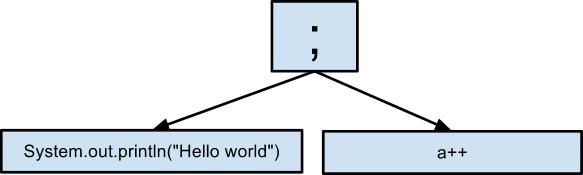
\includegraphics[width=0.8\textwidth]{seqTree}
	\caption{Последовательные операторы}
	\label{fig:seqImage}
\end{figure}

\begin{figure}[h!]
	\centering
	% \inputminted{c}{codes/seqCode1.java}
	\lstinputlisting[language=Java]{codes/seqCode1.java}
	\caption{Последовательные операторы в строчку}
	\label{fig:seqCode1}
\end{figure}

\begin{figure}[h!]
	\centering
	% \inputminted{c}{codes/seqCode2.java}
	\lstinputlisting[language=Java]{codes/seqCode2.java}
	\caption{Последовательные операторы в несколько строк}
	\label{fig:seqCode2}
\end{figure}


Рассмотрим другой пример.
Пусть нам нужно текстовое представление синтаксического дерева конструкции
“\lstinline{if}”, и заданы шаблоны c рис.~\ref{fig:ifTemplate2} и
\ref{fig:ifTemplate1}. При этом вариант, изображенный на
рис.~\ref{fig:ifTemplate2} выбирается только в случае, если условие и
ветки могут быть напечатаны в одну строчку.

\begin{figure}[h!]
	\subfloat[]{
		\lstinputlisting[language=Haskell]{codes/ifTemplate2.hs}
		\label{fig:ifTemplate2}	
	}
	\quad
	\subfloat[]{
		\lstinputlisting[language=Haskell]{codes/ifTemplate1.hs}
		\label{fig:ifTemplate1}	
	}
	\caption{Представления для конструкции “\lstinline{if}”}
\end{figure}


Тогда для деревьев, представленных на рис.
\ref{fig:ifImage1} и \ref{fig:ifImage2}, будут напечатаны коды с
рис. \ref{fig:ifCode1} и \ref{fig:ifCode2} соответственно.

\begin{figure}[h!]
	\subfloat[]{
		\centering
		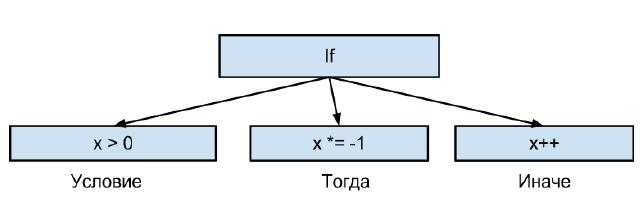
\includegraphics[width=0.6\textwidth]{if1}
		\label{fig:ifImage1}
	}
	\quad
	\subfloat[]{
		\centering
		% \inputminted{haskell}{codes/ifCode1.hs}
		\lstinputlisting[language=Haskell]{codes/ifCode1.hs}
		\label{fig:ifCode1}	
	}

	\caption{Использование представления с рис.~\ref{fig:ifTemplate2}}
\end{figure}

\begin{figure}[h!]
	\subfloat[]{
		\centering
		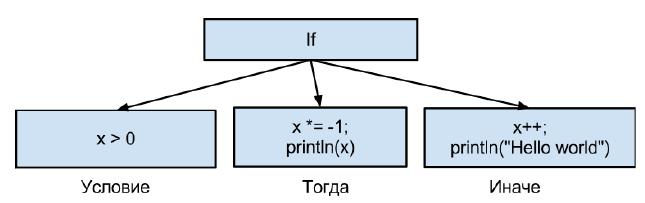
\includegraphics[width=0.6\textwidth]{if2}
		\label{fig:ifImage2}
	}
	\quad
	\subfloat[]{
		\centering
		% \inputminted{haskell}{codes/ifCode1.hs}
		\lstinputlisting[language=Haskell]{codes/ifCode2.hs}
		\label{fig:ifCode2}	
	}

	\caption{Использование представления с рис.~\ref{fig:ifTemplate1}}
\end{figure}

Существует несколько подходов к написанию принтеров.
Классическим способом задания принтеров в функциональных языках
программирования являются
принтер-комбинаторы~\cite{wadler, swierstra, swierstraChitil,
swierstra04, hughes, peytonJones, kiselyov, chitil, swiComb}.
Кроме того, существует работа, посвященная совместной разработке
принтера и синтаксического анализатора~\cite{rendelInvert}.
В \cite{jongeEveryOccasion, jongeReengine, brandBox} описаны методы
создания принтеров с помощью специализированных грамматик.

К сожалению, принтеры, создаваемые с помощью упомянутых подходов,
слабопараметризуемы и сложны. Чтобы избежать подобных проблем,
можно использовать шаблоны для описания представлений синтаксических
конструкций. Принципиальная возможность осуществления такого способа была
доказана в рамках предыдущей работы
автора. В \cite{myCoursePaper} был разработан
обобщенный принтер для учебного языка L, использующий расширяемый
синтаксический анализатор целевого языка для получения шаблонов.

Целью данной работы является разработка метода задания принтеров с помощью
образцов для языков программирования. 
Для апробирования метода было принято решение разработать принтер-плагин
языка Java для среды разработки IntelliJ IDEA\footnote{\cd{http://www.jetbrains.com/idea/}}.
В ходе разработки данного метода возникла необходимость улучшить существующую
принтер-комбинаторную библиотеку\cite{swierstra}. 

% Они вводят отношение \emph{частичного изоморфизма} на множествах абстрактных
% и конкретных синтаксических деревьев. Введение такого отношения позволяет
% совместно разрабатывать принтер и синтаксический анализатор. Кроме того,
% что таким образом уменьшается общий объем работы, подобный подход позволяет
% избежать несоответствия между принтером и анализатором.

% Вообще-то под \emph{комбинатором} понимается
% $\lambda$-терм без свободных переменных, но в нашем контексте о нем можно
% думать несколько проще --- как о функции высшего порядка,
% которая позволяет комбинировать сложный принтер из более простых.
